\documentclass[tikz,border=0pt,11pt]{standalone}
\usepackage[T1]{fontenc}
\usepackage[utf8]{inputenc}
\usepackage{lmodern,amsmath,amssymb}
\usepackage[swedish]{babel}
\usetikzlibrary{arrows.meta,calc,positioning,decorations.pathmorphing,decorations.pathreplacing,patterns,shadings}
\definecolor{navy}{HTML}{102F40}
\definecolor{teal}{HTML}{147D78}
\definecolor{lightteal}{HTML}{E6F1ED}
\definecolor{gold}{HTML}{B88B3B}
\definecolor{palegold}{HTML}{F7EEDB}
\definecolor{rust}{HTML}{B6533B}
\definecolor{palerust}{HTML}{FAEAE4}
\definecolor{paper}{HTML}{F7F5EE}
\definecolor{muted}{HTML}{5B6D72}
\definecolor{line}{HTML}{D6DED8}
\renewcommand{\familydefault}{\sfdefault}
\newcommand{\atom}[5]{\shade[ball color=#3!70] (#1,#2) circle (#5);\node[text=white,font=\bfseries\small] at (#1,#2){#4};}
\newcommand{\water}[3]{\begin{scope}[shift={(#1,#2)},scale=#3]\draw[navy!45,line width=2pt] (-.3,.22)--(0,0)--(.3,.22);\atom{0}{0}{rust}{O}{.22}\atom{-.3}{.22}{teal}{H}{.15}\atom{.3}{.22}{teal}{H}{.15}\end{scope}}
\newcommand{\panel}[4]{\filldraw[fill=white,draw=line,rounded corners=5pt] (#1,#2) rectangle ++(#3,#4);}
\newcommand{\note}[4]{\node[txt,text width=#3cm] at (#1,#2){#4};}
\tikzset{txt/.style={anchor=north west,align=left,text=navy,font=\small},
 head/.style={anchor=west,text=navy,font=\bfseries\large},
 label/.style={align=center,text=navy,font=\small},
 smalllabel/.style={align=center,text=muted,font=\footnotesize},
 arrow/.style={-{Latex[length=2.5mm,width=1.8mm]},line width=1.2pt,draw=teal},
 goldarrow/.style={-{Latex[length=2.5mm]},line width=1.2pt,draw=gold},
 rustarrow/.style={-{Latex[length=2.5mm]},line width=1.2pt,draw=rust},
 dashedarrow/.style={arrow,dashed},
 badge/.style={fill=lightteal,rounded corners=3pt,text=teal,font=\bfseries\small,inner sep=5pt}}
\begin{document}
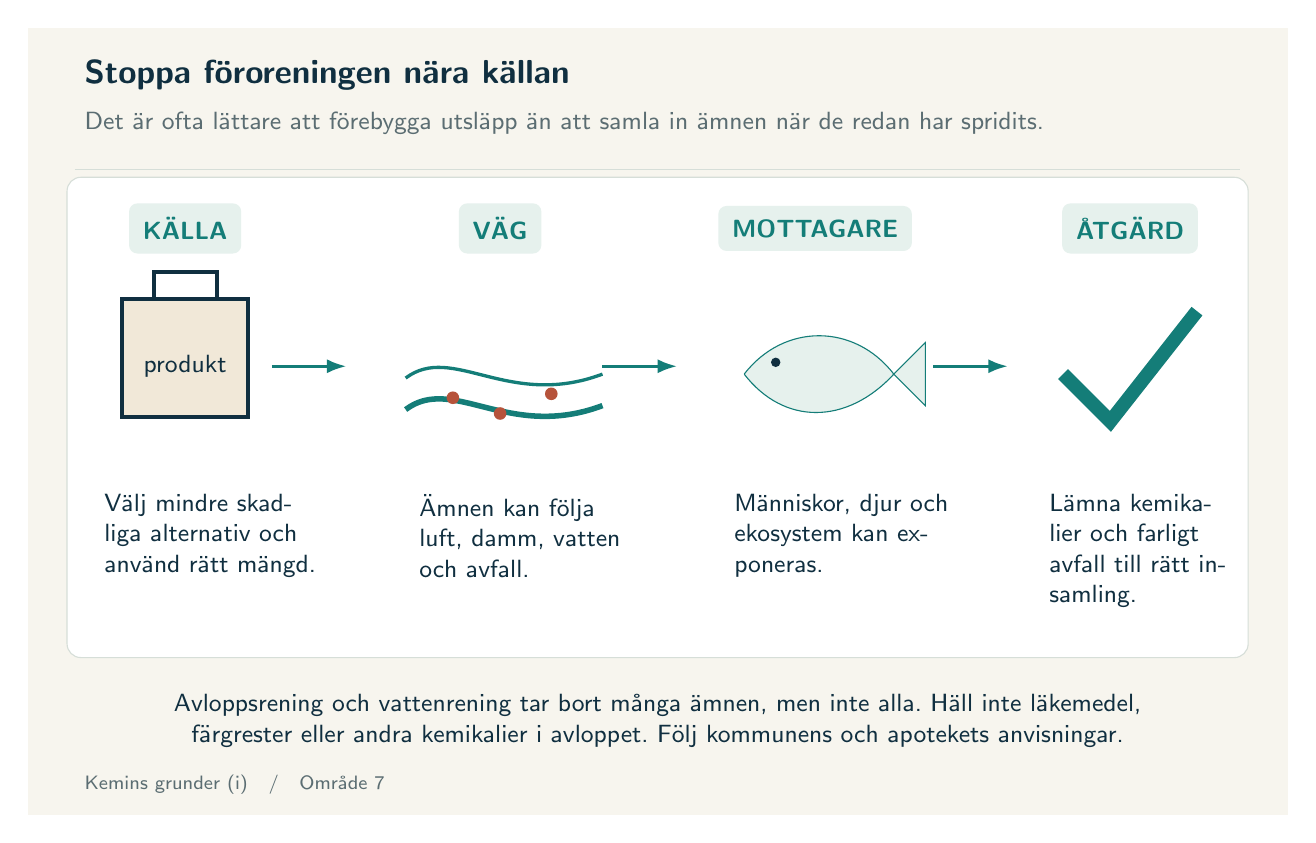
\begin{tikzpicture}[x=1cm,y=1cm]
\path[use as bounding box] (0,0) rectangle (16,10);
\fill[paper] (0,0) rectangle (16,10);
\node[head] at (.6,9.4){Stoppa föroreningen nära källan};
\note{.6}{9.05}{14.8}{\textcolor{muted}{Det är ofta lättare att förebygga utsläpp än att samla in ämnen när de redan har spridits.}}
\draw[line] (.6,8.2)--(15.4,8.2);

\panel{.5}{2}{15}{6.1}
\foreach \x/\title in {2/KÄLLA,6/VÄG,10/MOTTAGARE,14/ÅTGÄRD}{\node[badge] at (\x,7.45){\title};}
\draw[navy,fill=gold!20,line width=1.4pt] (1.2,5.05) rectangle(2.8,6.55);\draw[navy,line width=1.4pt] (1.6,6.55)--(1.6,6.9)--(2.4,6.9)--(2.4,6.55);\node[label] at (2,5.7){produkt};
\draw[teal,line width=2pt] (4.8,5.15)..controls(5.4,5.6)and(6.1,4.75)..(7.3,5.2);\draw[teal,line width=1.2pt] (4.8,5.55)..controls(5.4,6)and(6.1,5.15)..(7.3,5.6);\foreach \x/\y in {5.4/5.3,6/5.1,6.65/5.35}{\fill[rust] (\x,\y) circle(.08);}
\draw[teal,fill=lightteal] (9.1,5.6)..controls(9.6,6.25)and(10.5,6.25)..(11,5.6)..controls(10.4,4.95)and(9.6,4.95)..(9.1,5.6);\draw[teal,fill=lightteal] (11,5.6)--(11.4,6)--(11.4,5.2)--cycle;\fill[navy] (9.5,5.75) circle(.06);
\draw[teal,line width=5pt] (13.15,5.6)--(13.75,5)--(14.85,6.4);
\foreach \x in {3.1,7.3,11.5}{\draw[arrow] (\x,5.7)--++(.95,0);}
\note{.85}{4.2}{2.8}{Välj mindre skadliga alternativ och använd rätt mängd.}
\note{4.85}{4.2}{2.8}{Ämnen kan följa luft, damm, vatten och avfall.}
\note{8.85}{4.2}{2.8}{Människor, djur och ekosystem kan exponeras.}
\note{12.85}{4.2}{2.3}{Lämna kemikalier och farligt avfall till rätt insamling.}
\node[label,text width=14cm] at (8,1.2){Avloppsrening och vattenrening tar bort många ämnen, men inte alla. Häll inte läkemedel, färgrester eller andra kemikalier i avloppet. Följ kommunens och apotekets anvisningar.};\node[anchor=west,text=muted,font=\scriptsize] at (.6,.38){Kemins grunder (i)\quad /\quad Område 7};

\end{tikzpicture}\end{document}
